\documentclass[xetex,mathserif,serif]{beamer}
\usepackage{polyglossia}
\usepackage{minted}
\usepackage{tabu}

\usepackage{textpos}
\setlength{\TPHorizModule}{1cm}
\setlength{\TPVertModule}{1cm}

\useoutertheme{infolines}

\usepackage{fontspec}
\setmainfont{FreeSans}
\newfontfamily{\russianfonttt}{FreeSans}

\setbeamertemplate{blocks}[rounded][shadow=false]
\setbeamercolor*{block title example}{fg=green!50!black,bg=green!20}
\setbeamercolor*{block body example}{fg=black,bg=green!10}

\setbeamercolor*{block title alerted}{fg=red!50!black,bg=red!20}
\setbeamercolor*{block body alerted}{fg=black,bg=red!10}

\definecolor{cadmiumgreen}{rgb}{0.0, 0.42, 0.24}

\tabulinesep=0.7mm

\newcommand{\attribution}[1] {
\vspace{-5mm}\begin{flushright}\begin{scriptsize}\textcolor{gray}{\textcopyright\, #1}\end{scriptsize}\end{flushright}
}

\title{Глубокое метамоделирование}
\author[Юрий Литвинов]{Ю.В. Литвинов \newline 
	\textcolor{gray}{\small\texttt{y.litvinov@spbu.ru}}
}

\date{???}

\begin{document}

	\frame{\titlepage}

	\section{Введение}

	\begin{frame}
		\frametitle{О визуальных языках}
		\begin{itemize}
			\item Модели -- неформальные или формальные
			\item Языки моделирования: UML, IDEFx, BPMN, ...
			\item Языки визуального программирования: Simulink, LabView, ...
			\item Предметно-ориентированные визуальные языки: TRIK Studio, Robolab, Node-RED, ...
		\end{itemize}
		\begin{center}
			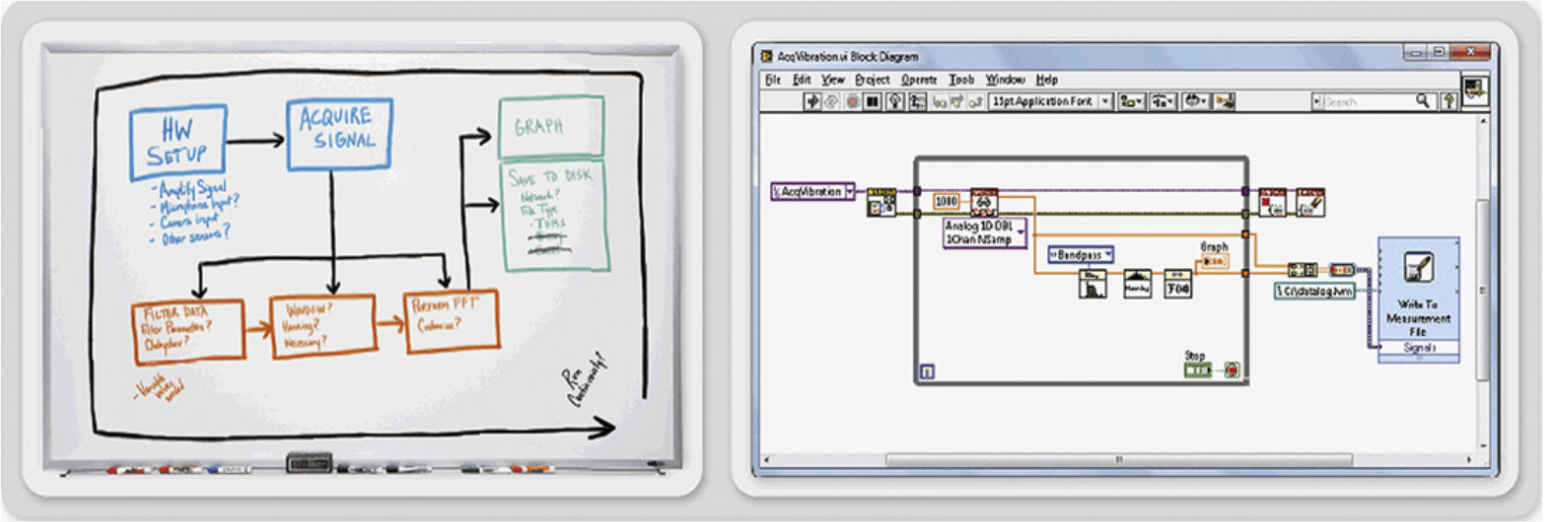
\includegraphics[width=0.8\textwidth]{sketchesVsFormalNotations.png}
			\attribution{N. Medvidovic}
		\end{center}
	\end{frame}

	\begin{frame}
		\frametitle{Язык UML}
		\begin{columns}
			\begin{column}{0.45\textwidth}
				\begin{itemize}
					\item Самый известный визуальный язык
					\item Появился в середине 90-х
					\item Не язык, а набор языков
					\item 14 разных видов диаграмм
					\item Единое описание, общее ``ядро'' языка
					\item Плохо с семантикой
					\item Использует метамоделирование для задания синтаксиса
				\end{itemize}
			\end{column}
			\begin{column}{0.55\textwidth}
				\begin{center}
					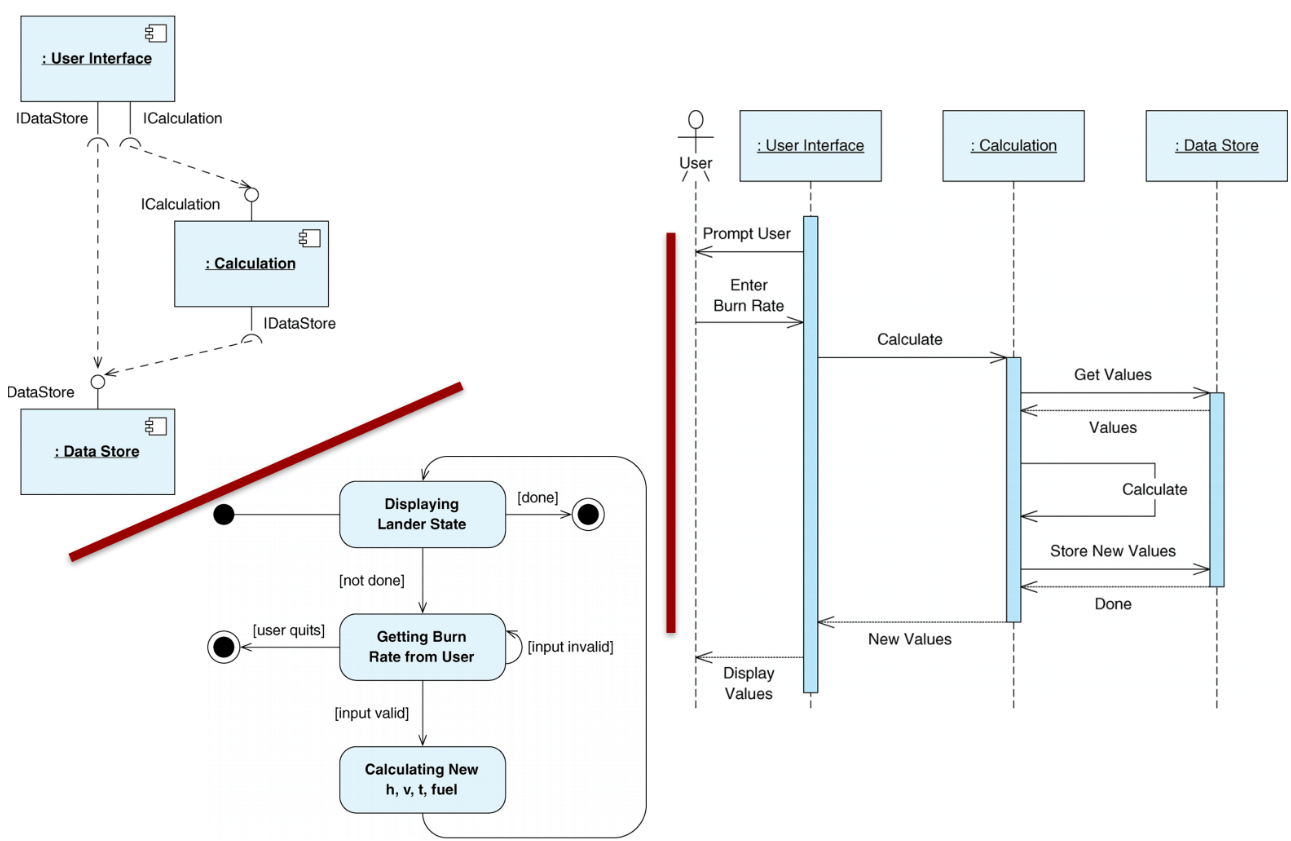
\includegraphics[width=0.8\textwidth]{uml.png}
					
					\vspace{5mm}
					
					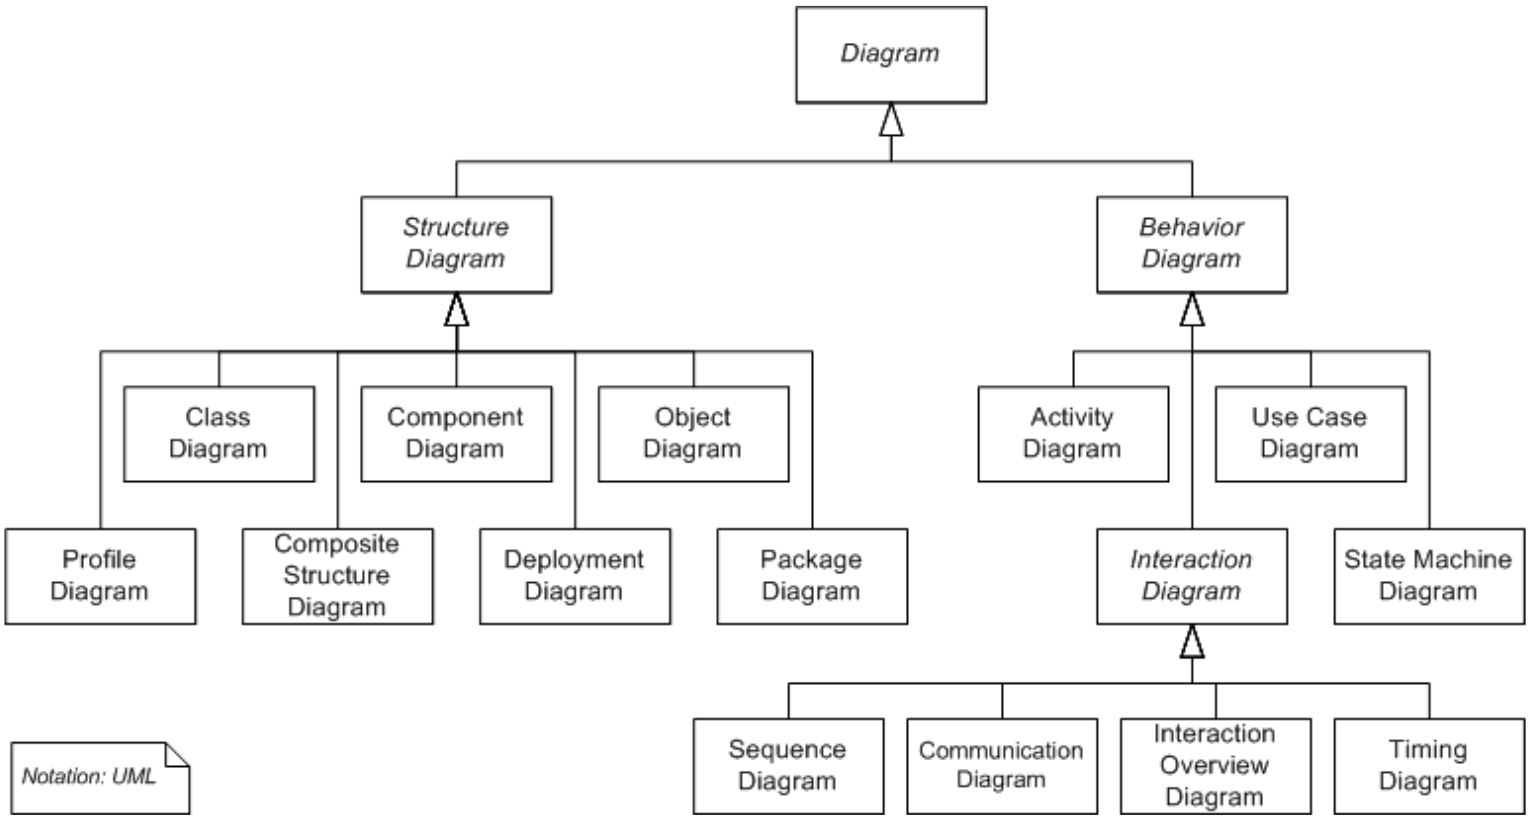
\includegraphics[width=0.8\textwidth]{umlDiagrams.png}
				\end{center}
			\end{column}
		\end{columns}
	\end{frame}

	\begin{frame}
		\frametitle{Метамоделирование}
		\begin{center}
			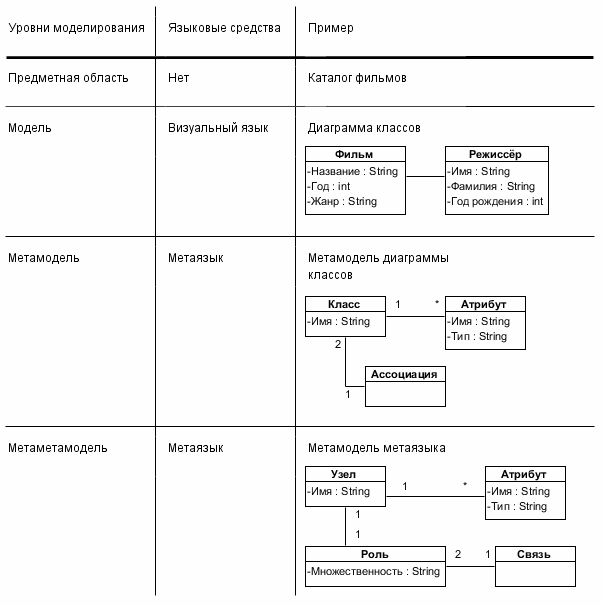
\includegraphics[width=0.6\textwidth]{metalevels.png}
		\end{center}
	\end{frame}

	\section{Проблемы с метамоделью UML}

	\begin{frame}
		\frametitle{Неоднозначность толкования ``instanceOf''}
		\framesubtitle{Пример}
		\begin{center}
			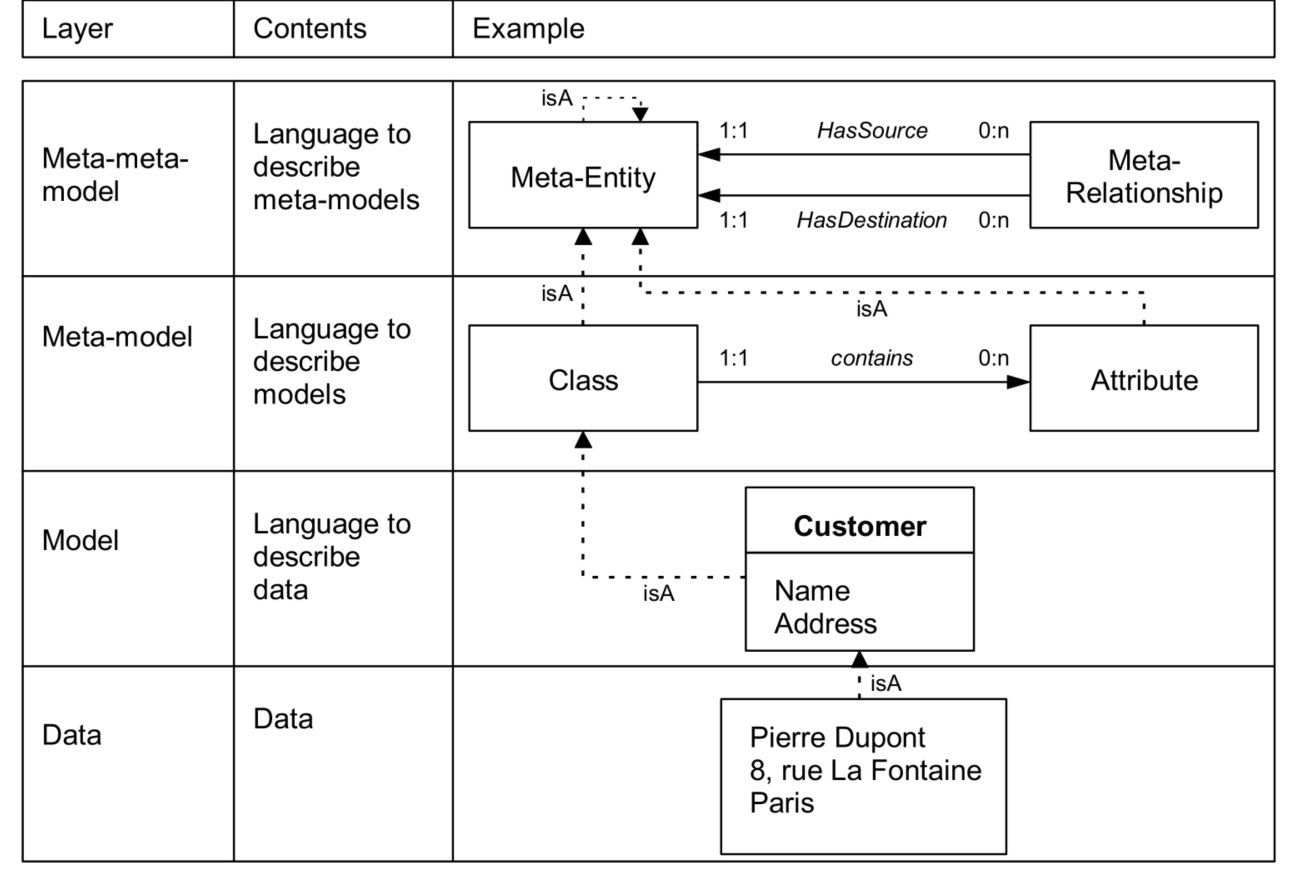
\includegraphics[width=0.7\textwidth]{bezivinExample.png}
			\attribution{J. Bezivin et al., Ontology-Based Layered Semantics for Precise OA\&D Modeling, 1997}
		\end{center}
	\end{frame}

	\begin{frame}
		\frametitle{Неоднозначность толкования ``instanceOf''}
		\framesubtitle{Собственно проблема}
		\begin{center}
			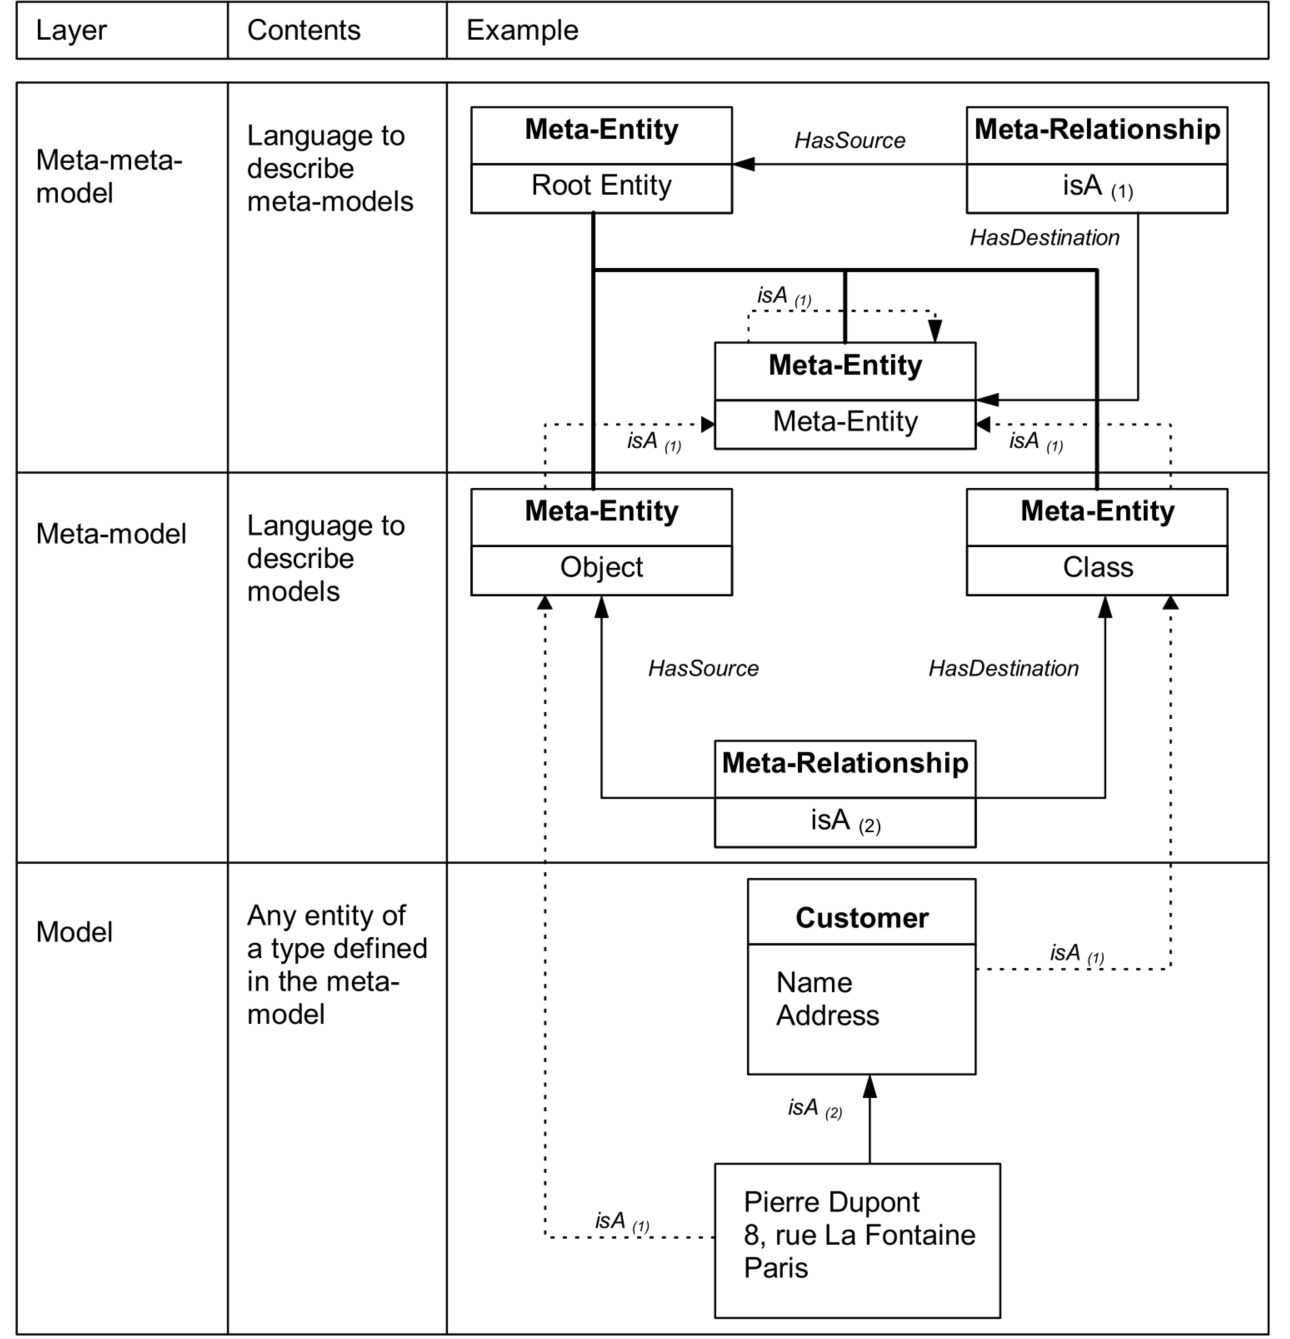
\includegraphics[width=0.55\textwidth]{bezivinIsA.png}
		\end{center}
	\end{frame}

\end{document}

